\subsection{Código de Huffman}
% harvard / HW3_ES250_sol_a.pdf

\begin{questions}
\question{
Considere a seguinte variável aleatória
\begin{equation}
        X = \left( \begin{matrix} 
        x_1  & x_2  & x_3  & x_4  & x_5  & x_6  & x_7 \\
        0.49 & 0.26 & 0.12 & 0.04 & 0.04 & 0.03 & 0.02
       \end{matrix}  \right)
\end{equation}

\begin{parts}
\part Encontre o código Huffman binário para $X$.
\part Qual é o comprimento esperado para este código?
\part Encontre o código Huffman ternário para $X$.
\part Qual é o comprimento esperado para este código?
\end{parts}
}

\begin{solution}
\begin{parts}
\part 
O código de Huffman é apresentado a seguir:

\begin{minipage}[b]{0.45\textwidth}
\tikzset{every tree node/.style={align=left,anchor=north,minimum width=2em,draw,circle},
         blank/.style={draw=none},
         edge from parent/.style=
         {draw, edge from parent path={(\tikzparentnode) -- (\tikzchildnode)}},
         every node/.append style={align=left},
         level distance=1.5cm}
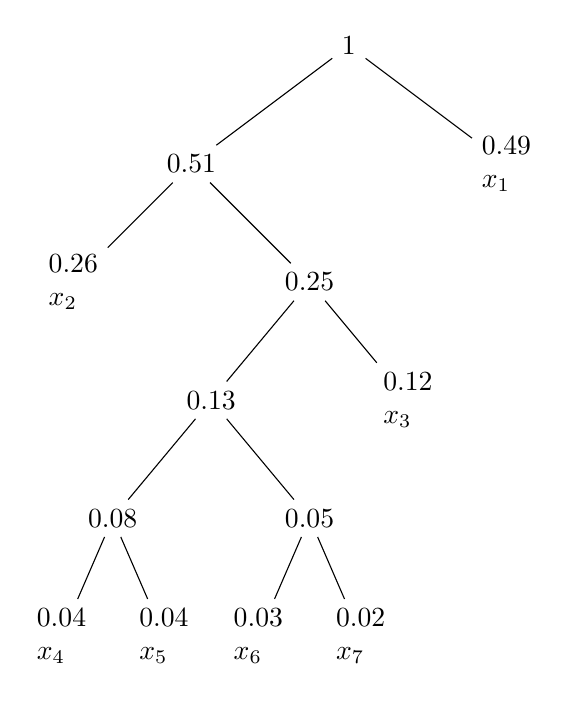
\begin{tikzpicture}[level distance=1.5cm,
  level 1/.style={sibling distance=4cm},
  level 2/.style={sibling distance=3cm},
  level 3/.style={sibling distance=2.5cm},
  level 4/.style={sibling distance=2.5cm},
  level 5/.style={sibling distance=1.3cm}]
  \node {1}
    child {
                node {0.51}
        child {node {0.26 \\ $x_2$}}
        child {node {0.25}
                child { 
                        node {0.13}
                        child {node {0.08} 
                                child {node {0.04 \\ $x_4$}}
                                child {node {0.04 \\ $x_5$}}
                        }
                        child {node {0.05}
                                        child {node {0.03 \\ $x_6$}}
                                        child {node {0.02 \\ $x_7$}}                            
                        }
                }
                child { node {0.12 \\ $x_3$} }
        }
        }
    child {
                node {0.49 \\ $x_1$}
    };
\end{tikzpicture}
\end{minipage}
  \hfill
\begin{minipage}[b]{0.45\textwidth}
\centering
   \begin{tabular}[b]{clc}
        símbolo & código & comprimento \\ \hline
        $x_1$ & 1 & 1\\
        $x_2$ & 00 & 2\\
        $x_3$ & 011 & 3\\
        $x_4$ & 01000 & 5\\
        $x_5$ & 01001 & 5\\
        $x_6$ & 01010 & 5\\
        $x_7$ & 01011 & 5
   \end{tabular}

\end{minipage}


\part 
   Comprimento esperado: 
   \begin{equation}
   L(C) = \sum_x p(x) l(x) = 2.02  .
   \end{equation}

   Entropia:
   \begin{equation}
   H(X) = - \sum_x p(x) \log p(x) = 2.0128 \text{bits} .
   \end{equation}



\part 
Para o código ternários, teremos:

\begin{minipage}[b]{0.45\textwidth}
\tikzset{every tree node/.style={align=left,anchor=north,minimum width=2em,draw,circle},
         blank/.style={draw=none},
         edge from parent/.style=
         {draw, edge from parent path={(\tikzparentnode) -- (\tikzchildnode)}},
         every node/.append style={align=left},
         level distance=1.5cm}
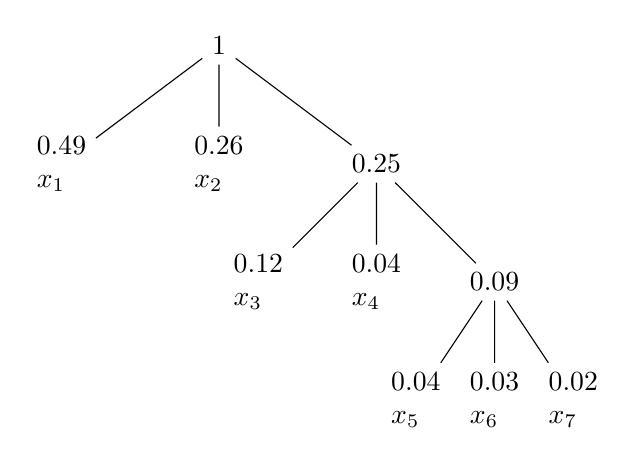
\begin{tikzpicture}[level distance=1.5cm,
  level 1/.style={sibling distance=2cm},
  level 2/.style={sibling distance=1.5cm},
  level 3/.style={sibling distance=1cm},
  level 5/.style={sibling distance=1cm}]
  \node {1}
        child { node {0.49 \\ $x_1$} }
        child { node {0.26 \\ $x_2$} }
        child { node {0.25} 
                child { node {0.12 \\ $x_3$} }
                child { node {0.04 \\ $x_4$} }
                child { node {0.09} 
                        child { node {0.04 \\ $x_5$} }
                        child { node {0.03 \\ $x_6$} }
                        child { node {0.02 \\ $x_7$} }
                }
        }
        ;
\end{tikzpicture}
\end{minipage}
  \hfill
\begin{minipage}[b]{0.45\textwidth}
\centering
   \begin{tabular}[b]{clc}
        símbolo & código & comprimento \\ \hline
        $x_1$ & 0 & 1\\
        $x_2$ & 1 & 1\\
        $x_3$ & 20 & 2\\
        $x_4$ & 21 & 2\\
        $x_5$ & 220 & 3\\
        $x_6$ & 221 & 3\\
        $x_7$ & 222 & 3
   \end{tabular}
\end{minipage}

\part 
   Comprimento esperado:
   \begin{equation}
   L(C) = \sum_x p(x) l(x) = 1.34  .
   \end{equation}

   Entropia:
   \begin{equation}
   H_3(X) = - \sum_x p(x) \log_3 p(x) = 1.2699 \text{trits} .
   \end{equation}

\end{parts}
\end{solution}
\end{questions}
